\documentclass[]{article}
\usepackage{lmodern}
\usepackage{amssymb,amsmath}
\usepackage{ifxetex,ifluatex}
\usepackage{fixltx2e} % provides \textsubscript
\ifnum 0\ifxetex 1\fi\ifluatex 1\fi=0 % if pdftex
  \usepackage[T1]{fontenc}
  \usepackage[utf8]{inputenc}
\else % if luatex or xelatex
  \ifxetex
    \usepackage{mathspec}
    \usepackage{xltxtra,xunicode}
  \else
    \usepackage{fontspec}
  \fi
  \defaultfontfeatures{Mapping=tex-text,Scale=MatchLowercase}
  \newcommand{\euro}{€}
\fi
% use upquote if available, for straight quotes in verbatim environments
\IfFileExists{upquote.sty}{\usepackage{upquote}}{}
% use microtype if available
\IfFileExists{microtype.sty}{%
\usepackage{microtype}
\UseMicrotypeSet[protrusion]{basicmath} % disable protrusion for tt fonts
}{}
\ifxetex
  \usepackage[setpagesize=false, % page size defined by xetex
              unicode=false, % unicode breaks when used with xetex
              xetex]{hyperref}
\else
  \usepackage[unicode=true]{hyperref}
\fi
\hypersetup{breaklinks=true,
            bookmarks=true,
            pdfauthor={Jonathan Werner},
            pdftitle={Bachelorarbeit - Better accuracy of automatic lecture transcriptions by using context information from slide contents},
            colorlinks=true,
            citecolor=blue,
            urlcolor=blue,
            linkcolor=magenta,
            pdfborder={0 0 0}}
\urlstyle{same}  % don't use monospace font for urls
\usepackage{longtable,booktabs}
\usepackage{graphicx,grffile}
\makeatletter
\def\maxwidth{\ifdim\Gin@nat@width>\linewidth\linewidth\else\Gin@nat@width\fi}
\def\maxheight{\ifdim\Gin@nat@height>\textheight\textheight\else\Gin@nat@height\fi}
\makeatother
% Scale images if necessary, so that they will not overflow the page
% margins by default, and it is still possible to overwrite the defaults
% using explicit options in \includegraphics[width, height, ...]{}
\setkeys{Gin}{width=\maxwidth,height=\maxheight,keepaspectratio}
\setlength{\parindent}{0pt}
\setlength{\parskip}{6pt plus 2pt minus 1pt}
\setlength{\emergencystretch}{3em}  % prevent overfull lines
\providecommand{\tightlist}{%
  \setlength{\itemsep}{0pt}\setlength{\parskip}{0pt}}
\setcounter{secnumdepth}{5}

\title{Bachelorarbeit - Better accuracy of automatic lecture transcriptions by
using context information from slide contents}
\author{Jonathan Werner}
\date{}
\usepackage[utf8]{inputenc}
\usepackage{hyperref}
\usepackage[all]{hypcap}

\usepackage{titlesec}
\newcommand{\sectionbreak}{\clearpage}

% Redefines (sub)paragraphs to behave more like sections
\ifx\paragraph\undefined\else
\let\oldparagraph\paragraph
\renewcommand{\paragraph}[1]{\oldparagraph{#1}\mbox{}}
\fi
\ifx\subparagraph\undefined\else
\let\oldsubparagraph\subparagraph
\renewcommand{\subparagraph}[1]{\oldsubparagraph{#1}\mbox{}}
\fi

\begin{document}
\maketitle

{
\hypersetup{linkcolor=black}
\setcounter{tocdepth}{3}
\tableofcontents
}
\newpage

\section*{Introduction}\label{introduction}
\addcontentsline{toc}{section}{Introduction}

Scannability is crucial for academic research: you have to be able to
quickly evaluate the usefulness of a given resource by skimming the
content and looking for the parts that are specifically relevant to the
task at hand.

The medium in which those resources are available is very centered on
textual representation. Spoken content, hereinafter called \emph{speech
media} (audio- or audiovisual media that mainly consists of spoken
language) doesn't make it possible to scan its contents. You are
``stabbing in the dark'' when looking for something specific in a medium
like this and have to consume it like a linear narrative.

This means that although lectures and conference talks are a central
element to science they are much more challenging and tedious to use for
research work.

Being able to a) efficiently search and b) look at the temporal
distribution of important keywords in a visually dense way would elevate
the usefulness of speech media in the scientific context immensely.

One approach to accomplish those goals is utilizing Automatic Speech
Recognition (ASR) to transcribe speech to text and also get timing
information for the recognized words. This makes it possible to derive
information about the density of given words at a given point of time in
the talk, which in turn allows to compute word occurence density maxima.
This opens up possibilities for compact visual representation of the
interesting keywords, thus allowing the user to scan.

The main challenge when using ASR for this task is the recognition
accuracy of technical terms. Most of them are not included in the
language models that are available as those are broad and generic so as
to optimize for accuracy over a wide topic spectrum. But when they are
not included into the language model they have no chance to be correctly
recognized at all.

So the usefulness of applying ASR with a generic language model to the
problem is very small, as the intersection of interesting keywords with
those technical terms that can not be recognized is very big.

The central goal of this thesis is to explore an approach to overcome
this problem. This approach consists of using words from lecture slides
or other notes to generate a lecture-specific language model. This is
then interpolated with a generic language model and being compared to
the `baseline' accuracy of the generic model.

\pagebreak

\subsection*{Structure of this thesis}\label{structure-of-this-thesis}
\addcontentsline{toc}{subsection}{Structure of this thesis}

The structure of this thesis is laid out as follows:

\begin{enumerate}
\def\labelenumi{(\arabic{enumi})}
\item
  \textbf{Research questions}

  I will state the research questions.
\item
  \textbf{Scientific Background}

  \begin{enumerate}
  \item
    I will start by giving an overview over the state of the art of ASR
    and the most prevalent approaches.
  \item
    I will explain the \emph{concepts} which are fundamental for the
    understanding of speech recognition.
  \item
    I will then examine the \emph{scientific work} that has been done on
    applying ASR to the problem of lectures transcriptions.
  \item
    Finally i will summarize the \emph{metrics} that have been used to
    assess the quality of the improvements in different approaches.
  \end{enumerate}
\item
  \textbf{Motivation}

  Here i will motivate why it is necessary to improve on the baseline
  performance of ASR in our context.

  I will talk about the role of keywords and technical terms and why
  they are not being detected and how that diminishes the usefulness of
  ASR for the purposes of scannability.
\item
  \textbf{Test data}

  I will use the openly available \emph{Open Yale Courses}
  {[}\hyperref[ref-openyale]{1}{]}, which provide a diverse selection of
  audio and video recordings of university lectures at Yale,
  additionally supplying quality manual transcriptions and course notes
  or slides.

  I will present the chosen courses, their selection criteria and
  discuss the range of types of lecture material.
\item
  \textbf{The LM-Interpolation approach}

  \begin{enumerate}
  \item
    \textbf{Technical basis}

    I will introduce the open source speech recognition framework
    \emph{Sphinx 4}. This is the software that is used for performing
    the actual recognition.
  \item
    \textbf{Process overview}

    I will then give a overview of the design and architecture of our
    approach.
  \item
    \textbf{Implementation}

    Finally i will describe the technical implementation by which the
    lecture material is compiled into a specialized language model and
    recognition is performed using a \emph{interpolated} language model.
  \end{enumerate}
\item
  \textbf{Analysis}

  \begin{enumerate}
  \item
    \textbf{Methods}

    I will discuss how to analyze the results and develop metrics that
    assess how well the given goals are met with our approach. 
  \item
    \textbf{Analysis}

    I will then perform quantitative analysis on our test dataset with
    the metrics we developed before.
  \item
    \textbf{Discussion, Finding and Conclusions}

    I will discuss the findings and draw conclusions from the
    quantitative analysis concerning the effectiveness of our approach.
  \end{enumerate}
\item
  \textbf{Visualization for Scannability}

  I will present a prototype visualization method that uses the results
  from our approach to present a condensed representation of the keyword
  content from lectures with the goal of providing a quick, interactive
  way to search and scan speech media.
\item
  \textbf{Improvements, Open Ends}

  I will discuss possible improvements and open ends that were out of
  the scope of this thesis but would be interesting to explore further.
\item
  \textbf{Summary}

  I will end by summarizing the goals, the proposed approach, the design
  and implementation, the analysis and the results.
\end{enumerate}

\pagebreak

\section{Research questions}\label{research-questions}

The central research questions i want to investigate in this thesis can
be formulated as follows:

\begin{enumerate}
\def\labelenumi{(\arabic{enumi})}
\item
  When we apply ASR to university lectures, what is the advantage of
  using an approach that consists of creating a lecture-specific
  language model and interpolating it with a generic language model,
  given that we are interested in improving the recognition accuracy of
  \emph{interesting keywords} for the sake of searchability and
  scannability?
\item
  What metric is useful for quantifying this advantage?
\end{enumerate}

A secondary question is: How can we \emph{use} the results from our
approach to provide graphical interfaces for improving the users ability
to search and scan the given speech medium?

The exploration of this question will not be the center of this thesis,
but it will provide practical motivation for the results that the
exploration.

\section{Background}\label{background}

\subsection{The field of Automatic Speech
Recognition}\label{the-field-of-automatic-speech-recognition}

Automatic Speech Recognition (ASR) can be defined as the process by
which a computer maps an acoustic speech signal to text
{[}\hyperref[ref-cmufaq]{2}{]}.

Rabiner and Juang {[}\hyperref[ref-rabiner]{3}{]} date the first
research on ASR back to the early 1950s, when Bell Labs built a system
for single-speaker digit recognition. Since then the field has seen
three major approaches, which Marquard {[}\hyperref[ref-marquard]{4}{]}
summarizes as follows:

\begin{quote}
\begin{enumerate}
\def\labelenumi{\arabic{enumi}.}
\tightlist
\item
  The \emph{acoustic-phonetic approach} aimed to identify features of
  speech such as vowels directly through their acoustic properties, and
  from there build up words based on their constituent phonetic
  elements.
\end{enumerate}
\end{quote}

\begin{quote}
\begin{enumerate}
\def\labelenumi{\arabic{enumi}.}
\setcounter{enumi}{1}
\tightlist
\item
  The \emph{statistical pattern-recognition approach} measures features
  of the acoustic signal, and compares these to existing patterns
  established from a range of reference sources to produce similarity
  scores which may be used to establish the best match.
\end{enumerate}
\end{quote}

\begin{quote}
\begin{enumerate}
\def\labelenumi{\arabic{enumi}.}
\setcounter{enumi}{2}
\tightlist
\item
  \emph{Artificial intelligence (AI) approaches} have been used to
  integrate different types of knowledge sources (such as acoustic,
  lexical, syntactic, semantic and pragmatic knowledge) to influence the
  output from a pattern-recognition system to select the most likely
  match.
\end{enumerate}
\end{quote}

The most prevalent approach today is the \emph{statistical
pattern-recognition approach}, as it produces results with much higher
accuracy compared to the acoustic-phonetic approach. The use of Hidden
Markov Models (HMM) has been playing a key role in this approach, as it
allows recognizers to use a statistical model of a given pattern rather
than a fixed representation.

In the last years there has been a resurgence of AI approaches,
specifically \emph{deep learning approaches}
{[}\hyperref[ref-hinton2012deep]{5}{]}. The ASR paradigm we will use for
this thesis will be limited to the former, however.

\subsection{Dimensions of speech
recognition}\label{dimensions-of-speech-recognition}

There are three dimensions which serve to classify different
applications of speech recognition {[}\hyperref[ref-cmufaq]{2}{]}
{[}\hyperref[ref-marquard]{4}{]}:

\begin{enumerate}
\def\labelenumi{(\arabic{enumi})}
\item
  \textbf{Dependent vs.~independent}. Dependent recognition systems are
  developed to be used by one speaker, whereas independent systems are
  developed to be used by \emph{any} speaker of a particular type, i.e
  North-American speakers. \textbf{Adaptive} systems lie between those
  poles, they are able to adapt to a particular speaker through
  training.
\item
  \textbf{Small vs.~large vocabulary}. Small vocabularies contain only
  up to a few hundred words and might be modeled by an explicit grammar,
  whereas large vocabularies contain tens of thousands of words so as to
  be able to model general purpose spoken language over a variety of
  domains.
\item
  \textbf{Continuous vs.~isolated speech}. Isolated speech consists of
  single words that are spoken with pauses in between them, whereas
  continuous speech consists of words that are spoken in a connected
  way. Continuous speech is significantly more difficult to recognize,
  as it is a) more difficult to find the start and end of words and b)
  the pronunciation of words changes in relation to their surrounding
  words.
\end{enumerate}

With those three dimensions we can for example classify the application
areas command and control systems, dictation and lecture transcription
{[}\hyperref[ref-marquard]{4}{]}:

\begin{longtable}[c]{@{}llll@{}}
\caption{Three application areas}\tabularnewline
\toprule
Application & Speaker & Vocabulary & Duration\tabularnewline
\midrule
\endfirsthead
\toprule
Application & Speaker & Vocabulary & Duration\tabularnewline
\midrule
\endhead
Dictation & Dependent & Large & Connected\tabularnewline
Command and control system & Independent & Small &
Isolated\tabularnewline
Lecture transcription & Independent & Large & Connected\tabularnewline
\bottomrule
\end{longtable}

The task of automatic lecture transcriptions can thus be characterized
as speaker-independent (SI) large continuous speech recognition (LVCSR).

\subsection{Concepts}\label{concepts}

Speech recognition in the \emph{statistical pattern-recognition
approach} paradigm has three major concepts necessary for its
understanding:

\begin{itemize}
\tightlist
\item
  phonemes
\item
  acoustic models (AM)
\item
  language models (LM)
\end{itemize}

\subsubsection{Phonemes}\label{phonemes}

A \emph{phoneme} is ``the smallest contrastive linguistic unit which may
bring about a change of meaning''
{[}\hyperref[ref-cruttenden2014gimson]{6}, p. 43{]}. They are the
smallest unit of sound in speech which are combined to form words. The
word \emph{sun} for example can be represented by the phonemes
\texttt{/s/}, \texttt{/u/} and \texttt{/n/}; the word \emph{table} by
\texttt{/t/}, \texttt{/a/} and \texttt{/bl/}.

A language together with a specific accent can be described by a set of
phonemes that it consists of. Figure \ref{phonemic-chart} uses symbols
from the International Phonetic Alphabet (IPA) to display the 44
phonemes that are being used in Received Pronunciation (RP), which is
regarded as the ``standard accent'' in the south of the United Kingdom
{[}\hyperref[ref-stevenson2011concise]{7}{]}.

\begin{figure}[htbp]
\centering
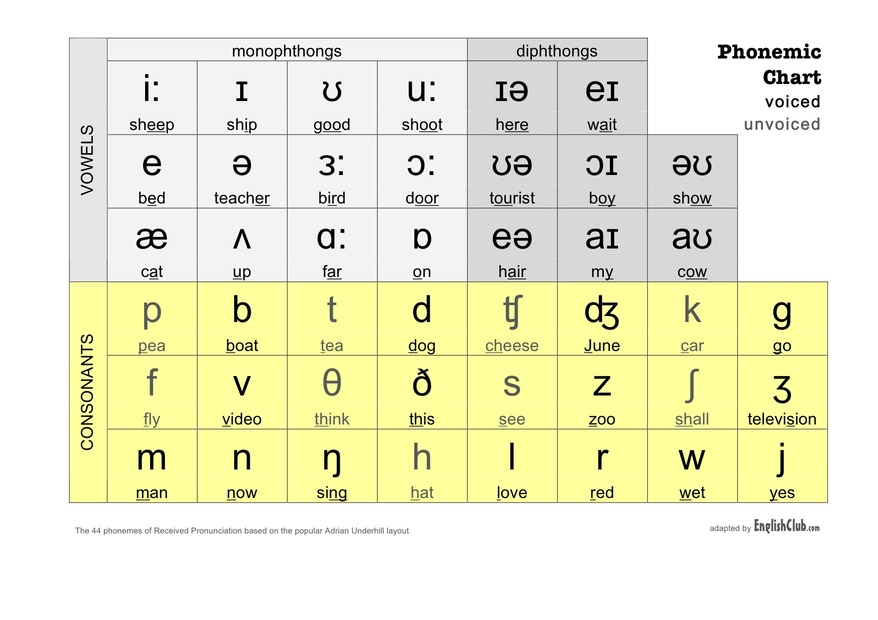
\includegraphics{images/phonemes_50.jpg}
\caption{Phonemic Chart representing 44 phonemes used in RP British
English\label{phonemic-chart}}
\end{figure}

To be able to use phonemes in software, an ASCII representation is more
suitable. The standard for General American English is the
\emph{Arpabet}. Here each phoneme is mapped to one or two capital
letters. The digits \texttt{0}, \texttt{1} and \texttt{2} signify stress
markers: no stress, primary and secondary stress respectively. A
comparison of the IPA format and the arphabet format can be seen in
Figure \ref{arpabet}, an excerpt that just shows the
\emph{monophthongs}.\footnote{pure vowel sounds with relatively fixed
  articulation at the start and the end that don't glide towards a new
  position of articulation}

\begin{figure}[htbp]
\centering
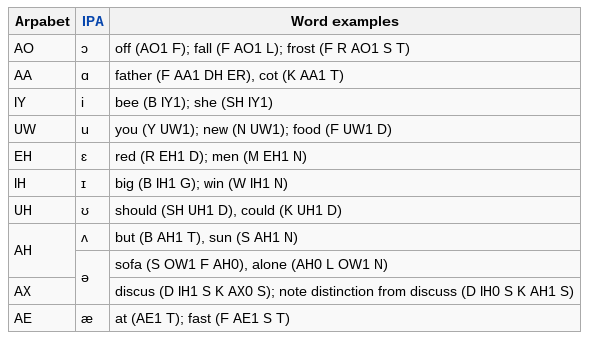
\includegraphics{images/arpabet.png}
\caption{Excerpt from the Arpabet {[}\hyperref[ref-wikiArpabet]{8}{]}
\label{arpabet}}
\end{figure}

\subsubsection{Acoustic models}\label{acoustic-models}

An acoustic model describes the statistical relation between an audio
signal and the probability that this signal represents a given phoneme.

Acoustic models are created by \emph{training} them on a \emph{corpus}
of audio recordings and matching transcripts. When being used in the
context of speaker-independent recognition, those models are trained
with a variety of speakers that represent a broad spectrum of the
language/accent that the acoustic model should represent.

Acoustic models alone are not sufficient for speech recognition, as they
do not have the higher-level linguistic information necessary to for
example decide between homonyms and similar-sounding phrases such as
``wreck a nice beach'' and ``recognize speech''
{[}\hyperref[ref-marquard]{4}, p. 11{]}. This information finally is
provided by \emph{Language Models}.

\subsubsection{Language Models}\label{language-models}

\newpage

\section*{Bibliography}\label{bibliography}
\addcontentsline{toc}{section}{Bibliography}

\hyperdef{}{ref-openyale}{\label{ref-openyale}}
{[}1{]} ``Open yale courses website.'' \url{http://oyc.yale.edu/}.

\hyperdef{}{ref-cmufaq}{\label{ref-cmufaq}}
{[}2{]} ``Comp.speech frequently asked questions.''
\url{http://www.speech.cs.cmu.edu/comp.speech/Section6/Q6.1.html}.

\hyperdef{}{ref-rabiner}{\label{ref-rabiner}}
{[}3{]} L. Rabiner and B.-H. Juang, ``Fundamentals of speech
recognition,'' 1993.

\hyperdef{}{ref-marquard}{\label{ref-marquard}}
{[}4{]} S. Marquard, ``Improving searchability of automatically
transcribed lectures through dynamic language modelling,'' 2012.

\hyperdef{}{ref-hinton2012deep}{\label{ref-hinton2012deep}}
{[}5{]} G. Hinton, L. Deng, D. Yu, G. E. Dahl, A.-r. Mohamed, N. Jaitly,
A. Senior, V. Vanhoucke, P. Nguyen, T. N. Sainath, and others, ``Deep
neural networks for acoustic modeling in speech recognition: The shared
views of four research groups,'' \emph{Signal Processing Magazine,
IEEE}, vol. 29, no. 6, pp. 82--97, 2012.

\hyperdef{}{ref-cruttenden2014gimson}{\label{ref-cruttenden2014gimson}}
{[}6{]} A. Cruttenden, \emph{Gimson's pronunciation of english}.
Routledge, 2014.

\hyperdef{}{ref-stevenson2011concise}{\label{ref-stevenson2011concise}}
{[}7{]} A. Stevenson and M. Waite, \emph{Concise oxford english
dictionary: Book \& cD-rOM set}. Oxford University Press, 2011.

\hyperdef{}{ref-wikiArpabet}{\label{ref-wikiArpabet}}
{[}8{]} ``English wikipedia arpabet article.''
\url{https://en.wikipedia.org/wiki/Arpabet}, 2015 (accessed 22.8.15).

\end{document}
